\chapter{Conclusions And Future Works}
\label{cha:conclusions}

In this chapter we will conclude our work, giving some general considerations about what we have done and some possible future works. 

\section{Conclusions}
\label{sec:conclusions}
In this work we have presented the problem of analyzing Chest X-Rays to automatically classify some pathologies. Starting from some works that were previously carried out by the scientific community, we developed a system able to achieve a mean AUROC across five different diseases of 0.902. Although Pham et al. \cite{pham2019interpreting} in their work obtained a better result, we introduced some novelties. 

\vspace{5mm}

Starting from the techniques proposed by the related works mentioned above, we developed multiple models using U-Ones and Label Smooth Regularization to deal with uncertain labels and Conditional Training to exploit diseases hierarchy. Then we investigated different approaches to aggregate the different models, showing that, instead of making a simple average of the predictions, the use of a weighted average, based on models' entropy, can improve the ensemble performance. Then, using the embeddings extracted by means of the \acp{CNN}, we showed that is possible, taking less time and computational resources, to build a system able to reach (or even surpass) the performance obtained by neural networks. Then, using the confusion matrices we tried, differently from other works, to give a more comprehensible vision of our model's output, showing exactly the number of correct and incorrect predictions, allowing also the system to abstain in case it is very uncertain about its diagnosis. 
Finally, for what it concern the pathologies visualization, we tried to improve it by aggregating the different Class Activation Maps produced by the models and we proposed a system to automatically extract a bounding box surrounding the region that most probably is interested by the disease. 

\section{Future Works}
\label{sec:future_works}
We will now talk about some approaches that could be investigated to improve this work.


\vspace{5mm}

In our research we tried to build a model that was as general as possible. However Pham et al. \cite{pham2019interpreting}, in their work, used some performance tweaking that allow their model to achieve very high results, with the downside of losing some generalization capability. It could be interesting to check whether those performance tweaking would actually lead to a better result or not.

\vspace{5mm}
For what it concern data, as we already said in Chapter \ref{cha:third_chapter}, during the preprocessing we discarded some informations related to the patients, such as its age and gender. These data instead, could be leveraged, trying to check if, giving them as additional input to a model, is possible to enhance the predictions. 
Moreover, in our work we only employed the frontal CXR, but the dataset we used comes with a pretty large number of Lateral CXR. A system able to process both a Frontal and a Lateral view would probably be able to better discriminate among the different diseases. 

\vspace{5mm}

Moreover, as we have seen, one of the biggest issues related to Chexpert dataset is that it's quite unbalanced, causing the perfomance of the less represented class to be worse than the other. Using some class balancing algorithm could produce an overall improvement.
For what it concern data, finally, it is worth noting that it exist a dataset whose \acp{CXR} have been labelled using the same approach employed in Chexpert \cite{johnson2019mimiccxrjpg}, containing almost 370 thousand additional images that could be used to train the models (with the downside that this approach requires more time and computational resources)

\vspace{5mm}

As we already told, the embeddings are able to capture the meaningful information needed to identify the presence or absence of a disease, with the advantage of drastically reducing the input dimension. In our work we used them to train Random Forest and XGBoost. However, given the small dimension of the embeddings (compared to that of the original images), it would be possible to investigate any other Machine Learning algorithm, even those that initially seemed to be not suitable for solving the task of CXR image analysis.

\vspace{5mm}

Once the embeddings have been extracted, moreover, they could be used to train models able to find any other pathology, not only those present in CheXpert. As proof of concept, we used them to identify the Chest X-Rays affected by SARS-CoV-2, the virus causing a pandemic that, starting from December 2019, spread all over the world. Using our trained \acp{CNN}, we extracted the embeddings of almost one hundred \acp{CXR} coming from sick patients and we used them to train a binary classifier using XGBoost, with the aim of distinguishing a regular Pneumonia (whose corresponding \acp{CXR} were already provided by CheXpert) from one caused by SARS-CoV-2. We used 10-fold cross validation as evaluation approach, obtaining the results in Table \ref{table:table_6.1}.

\vspace{5mm}

\begin{table}[h!]
\centering
\begin{tabular}{|l|l|l|} 
\hline
\textbf{Fold} & \textbf{Accuracy} & \textbf{AUROC} \\
\hline
Fold-1  &1.000 & 1.000\\ \hline
Fold-2  &0.947 & 0.929\\ \hline
Fold-3  &0.947 & 0.955\\\hline
Fold-4  &1.000 & 1.000\\\hline
Fold-5  &0.947 & 0.944\\\hline
Fold-6  &0.947 & 0.944\\\hline
Fold-7  &0.895 & 0.889\\\hline
Fold-8  &1.000 & 1.000\\\hline
Fold-9  &0.947 & 0.944\\\hline
Fold-10 &1.000 & 1.000\\\hline

\rowcolor[rgb]{0.851,0.851,0.851}AVG & 0.963 & 0.961\\
\hline
\end{tabular}

\caption[COVID-19 results]{COVID-19 Accuracy and AUROC of the 10 folds.}
\label{table:table_6.1}
\end{table}

\vspace{3mm}

As we can see, we obtained an average AUROC of 0.961 without using the full images, but exploiting only the embeddings. In some cases the model is able to perfectly distinguish the two diseases, as we can see in the confusion matrix reported \ref{fig:figure_6.1}.

\vspace{5mm}

\begin{figure}[htbp!]
\centering
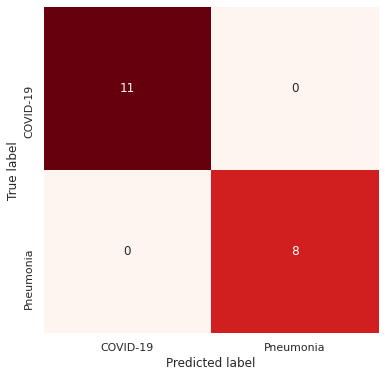
\includegraphics[scale=0.62]{Tesi/images/COVID CM.png}
\caption{COVID-19 Confusion Matrix}
\label{fig:figure_6.1}
\end{figure}

\newpage
\vspace{5mm}
Finally, the last approach we want to propose is that of using the bounding box that we generated to extract the area interested by the pathology and use it as input to the model, in order to let it focus its attention on a smaller region of the image.

